\documentclass[aspectratio=169]{beamer}
\usepackage[utf8]{inputenc}
\usepackage[T1]{fontenc}
\usepackage{graphicx}
\usepackage{amsmath}
\usepackage{amsfonts}
\usepackage{amssymb}
\usepackage{xcolor}
\usepackage{tikz}
\usepackage{booktabs}
\usepackage{array}
\usepackage{listings}
\usepackage{hyperref}

% Theme and colors
\usetheme{Madrid}
\usecolortheme{default}
\definecolor{mistralblue}{RGB}{0,102,204}
\definecolor{mistrallight}{RGB}{102,178,255}
\setbeamercolor{structure}{fg=mistralblue}
\setbeamercolor{frametitle}{fg=white,bg=mistralblue}

% Title page
\title[PII Masking with Mistral AI]{PII Masking Evaluation Framework}
\subtitle{Comparing Prompting, Fine-tuning, and Token Classification Approaches}
\author{Applied AI Engineer - Mistral AI Take-Home Project}
\date{\today}

\begin{document}

% Title slide
\begin{frame}
\titlepage
\end{frame}

% Outline
\begin{frame}{Outline}
\tableofcontents
\end{frame}

\section{Use Case \& Business Opportunities}

\begin{frame}{PII Masking: A Critical Business Need}
\begin{columns}
\begin{column}{0.6\textwidth}
\textbf{Why PII Masking?}
\begin{itemize}
\item \textbf{Privacy Compliance}: GDPR, HIPAA, CCPA requirements
\item \textbf{Data Security}: Protect sensitive information in processing pipelines
\item \textbf{Document Processing}: Automated anonymization of legal/financial documents
\end{itemize}

\vspace{0.5cm}
\textbf{Market Opportunities}
\begin{itemize}
\item Healthcare: Patient record processing
\item Finance: KYC document analysis
\item Legal: Contract and litigation support
\item Enterprise: HR document processing
\end{itemize}
\end{column}
\begin{column}{0.4\textwidth}
\begin{center}
\includegraphics[width=\textwidth]{images/pii_use_cases.png}
\end{center}
\end{column}
\end{columns}
\end{frame}

\begin{frame}{Business Impact \& Value Proposition}
\begin{columns}
\begin{column}{0.5\textwidth}
\textbf{Compliance Benefits}
\begin{itemize}
\item Automated GDPR Article 17 (Right to be forgotten)
\item HIPAA-compliant data processing
\item Reduced legal liability
\item Audit trail and documentation
\end{itemize}

\textbf{Operational Efficiency}
\begin{itemize}
\item 95\% reduction in manual review time
\item Real-time processing capabilities
\item Multi-PII support (54 PII classes)
\item Scalable cloud deployment
\end{itemize}
\end{column}
\begin{column}{0.5\textwidth}
\textbf{Cost Analysis}
\begin{itemize}
\item Manual review: \$40-60/hour
\item API approach: \$0.05-0.15/prediction
\item Fine-tuning: \$50-100 initial + \$0.02/prediction
\item Token classification: ~0$/prediction
\item Break-even: ~1,000 predictions/month
\end{itemize}

\vspace{0.3cm}
\begin{alertblock}{ROI Projection}
For enterprise clients processing 10k+ documents/month:
\textbf{60-80\% cost reduction} vs. manual processes
\end{alertblock}
\end{column}
\end{columns}
\end{frame}

\section{Dataset \& Evaluation Framework}

\begin{frame}{AI4Privacy PII-200k Dataset}
\begin{columns}
\begin{column}{0.6\textwidth}
\textbf{Dataset Overview}
\begin{itemize}
\item \textbf{Size}: 42k English samples,
\item \textbf{PII Classes}: 54 comprehensive categories
\item \textbf{Quality}: Human-validated synthetic data
\item \textbf{Privacy-Safe}: No real PII exposure in the dataset
\end{itemize}

\vspace{0.3cm}
\textbf{Key Features}
\begin{itemize}
\item Exact character-level annotations
\item Privacy masks with placeholders
\item Diverse text domains and contexts
\end{itemize}
\end{column}
\begin{column}{0.4\textwidth}
\begin{center}
\includegraphics[width=\textwidth]{images/dataset_distribution.png}
\caption{PII Class Distribution}
\end{center}
\end{column}
\end{columns}
\end{frame}

\begin{frame}{Dataset Example}
\begin{block}{Original Text}
\texttt{"Hi, my name is John Smith and my email is john.smith@company.com. I live at 123 Main Street, New York, NY 10001. My phone number is (555) 123-4567."}
\end{block}

\begin{block}{Ground Truth Annotations}
\begin{itemize}
\item \texttt{[15:25]} → \textcolor{red}{FIRSTNAME}: "John Smith"
\item \texttt{[42:65]} → \textcolor{blue}{EMAIL}: "john.smith@company.com"
\item \texttt{[78:94]} → \textcolor{green}{STREET}: "123 Main Street"
\item \texttt{[96:104]} → \textcolor{orange}{CITY}: "New York"
\item \texttt{[106:108]} → \textcolor{purple}{STATE}: "NY"
\item \texttt{[109:114]} → \textcolor{brown}{ZIPCODE}: "10001"
\item \texttt{[135:149]} → \textcolor{red}{PHONENUMBER}: "(555) 123-4567"
\end{itemize}
\end{block}

\begin{block}{Evaluation Challenge}
\textbf{Exact Position Matching}: Entities must match both \textit{type} AND \textit{exact character positions} to be considered correct.
\end{block}
\end{frame}

\section{Approach 1: LLM Prompting}

\begin{frame}{Mistral API Prompting Approach}
\begin{columns}
\begin{column}{0.6\textwidth}
\textbf{Core Strategy}
\begin{itemize}
\item \textbf{Structured Output}: JSON format for entity extraction
\item \textbf{Text Preservation}: No text rewriting, only entity identification
\item \textbf{Position Accuracy}: Regex matching for exact positioning
\item \textbf{Zero/Few-shot Learning}: Adaptable to new domains
\end{itemize}

\vspace{0.3cm}
\textbf{Why JSON over Text Rewriting?}
\begin{itemize}
\item Faster processing (no full text generation)
\item No transcription errors
\item Preserves original formatting/typos
\item Easier post-processing pipeline
\end{itemize}
\end{column}
\begin{column}{0.4\textwidth}
\begin{block}{JSON Output Format}
\begin{lstlisting}[language=json,basicstyle=\tiny]
{
  "PII": {
    "FIRSTNAME": ["John"],
    "EMAIL": ["john@company.com"],
    "STREET": ["123 Main St"],
    "PHONENUMBER": ["555-123-4567"]
  }
}
\end{lstlisting}
\end{block}

\vspace{0.3cm}
\begin{center}
\includegraphics[width=0.9\textwidth]{images/prompting_flow.png}
\end{center}
\end{column}
\end{columns}
\end{frame}

\begin{frame}{Mistral Models Comparison}
\begin{table}[h]
\centering
\begin{tabular}{lccc}
\toprule
\textbf{Model} & \textbf{Parameters} & \textbf{Cost/1M tokens} & \textbf{Use Case} \\
\midrule
mistral-small-latest & 22B & \$0.20 & Cost-effective baseline \\
mistral-medium-latest & - & \$2.70 & Balanced performance \\
mistral-large-latest & 123B & \$8.00 & Maximum accuracy \\
\bottomrule
\end{tabular}
\end{table}

\vspace{0.5cm}

\begin{columns}
\begin{column}{0.5\textwidth}
\textbf{Configuration}
\begin{itemize}
\item Max tokens: 1000
\item Batch inference for efficiency
\item Retry logic with exponential backoff
\end{itemize}
\end{column}
\begin{column}{0.5\textwidth}
\textbf{Prompt Engineering}
\begin{itemize}
\item System prompt with PII definitions
\item Structured output instructions
\item Few-shot examples (0-3 shots)
\end{itemize}
\end{column}
\end{columns}
\end{frame}

\begin{frame}{Evaluation Metrics \& Methodology}
\begin{columns}
\begin{column}{0.5\textwidth}
\textbf{Strict Position Matching}
\begin{itemize}
\item \textbf{True Positive}: Exact type + position match
\item \textbf{False Positive}: Predicted but incorrect/misplaced
\item \textbf{False Negative}: Missed entity
\item \textbf{No Partial Credit}: Position mismatch = error
\end{itemize}

\vspace{0.3cm}
\textbf{Metrics Calculated}
\begin{align}
\text{Precision} &= \frac{TP}{TP + FP} \\
\text{Recall} &= \frac{TP}{TP + FN} \\
\text{F1-Score} &= \frac{2 \cdot P \cdot R}{P + R}
\end{align}
\end{column}
\begin{column}{0.5\textwidth}
\textbf{Per-Class Analysis}
\begin{itemize}
\item F1-score for each PII type
\item Class-specific precision/recall
\item Error analysis by entity complexity
\item Performance vs. entity frequency
\end{itemize}

\vspace{0.3cm}
\begin{alertblock}{Token-Level Alignment}
Predictions aligned at character level, then validated against ground truth spans using exact boundary matching.
\end{alertblock}
\end{column}
\end{columns}
\end{frame}

\begin{frame}{Prompting Results: Zero-shot vs Few-shot}
\begin{columns}
\begin{column}{0.6\textwidth}
\begin{center}
\includegraphics[width=\textwidth]{images/prompting_results.png}
\end{center}
\end{column}
\begin{column}{0.4\textwidth}
\textbf{Key Findings}
\begin{itemize}
\item Few-shot learning: +15\% F1-score improvement
\item Consistent across all model sizes
\end{itemize}

\vspace{0.3cm}
\begin{table}[h]
\centering
\scriptsize
\begin{tabular}{lcc}
\toprule
\textbf{Approach} & \textbf{F1} & \textbf{Precision} \\
\midrule
Zero-shot & 0.734 & 0.821 \\
3-shot & 0.847 & 0.889 \\
5-shot & 0.852 & 0.891 \\
\bottomrule
\end{tabular}
\end{table}
\end{column}
\end{columns}
\end{frame}

\section{Approach 2: Fine-tuning}

\begin{frame}{Mistral Fine-tuning Strategy}
\begin{columns}
\begin{column}{0.6\textwidth}
\textbf{Fine-tuning Approach}
\begin{itemize}
\item \textbf{Base Model}: Mistral-8B-latest
\item \textbf{Task Format}: Same JSON structure as prompting
\item \textbf{System Prompt}: Reduced for efficiency
\item \textbf{Training Data}: 5k curated examples
\item \textbf{Validation}: 1k held-out examples
\end{itemize}

\vspace{0.3cm}
\textbf{Training Configuration}
\begin{itemize}
\item Learning Rate: 1e-4
\item Training Steps: 500
\end{itemize}
\end{column}
\begin{column}{0.4\textwidth}
\begin{center}
\includegraphics[width=\textwidth]{images/training_loss.png}
\caption{Training Loss Curve}
\end{center}
\end{column}
\end{columns}
\end{frame}

\begin{frame}{Fine-tuning Results \& Comparison}
\begin{center}
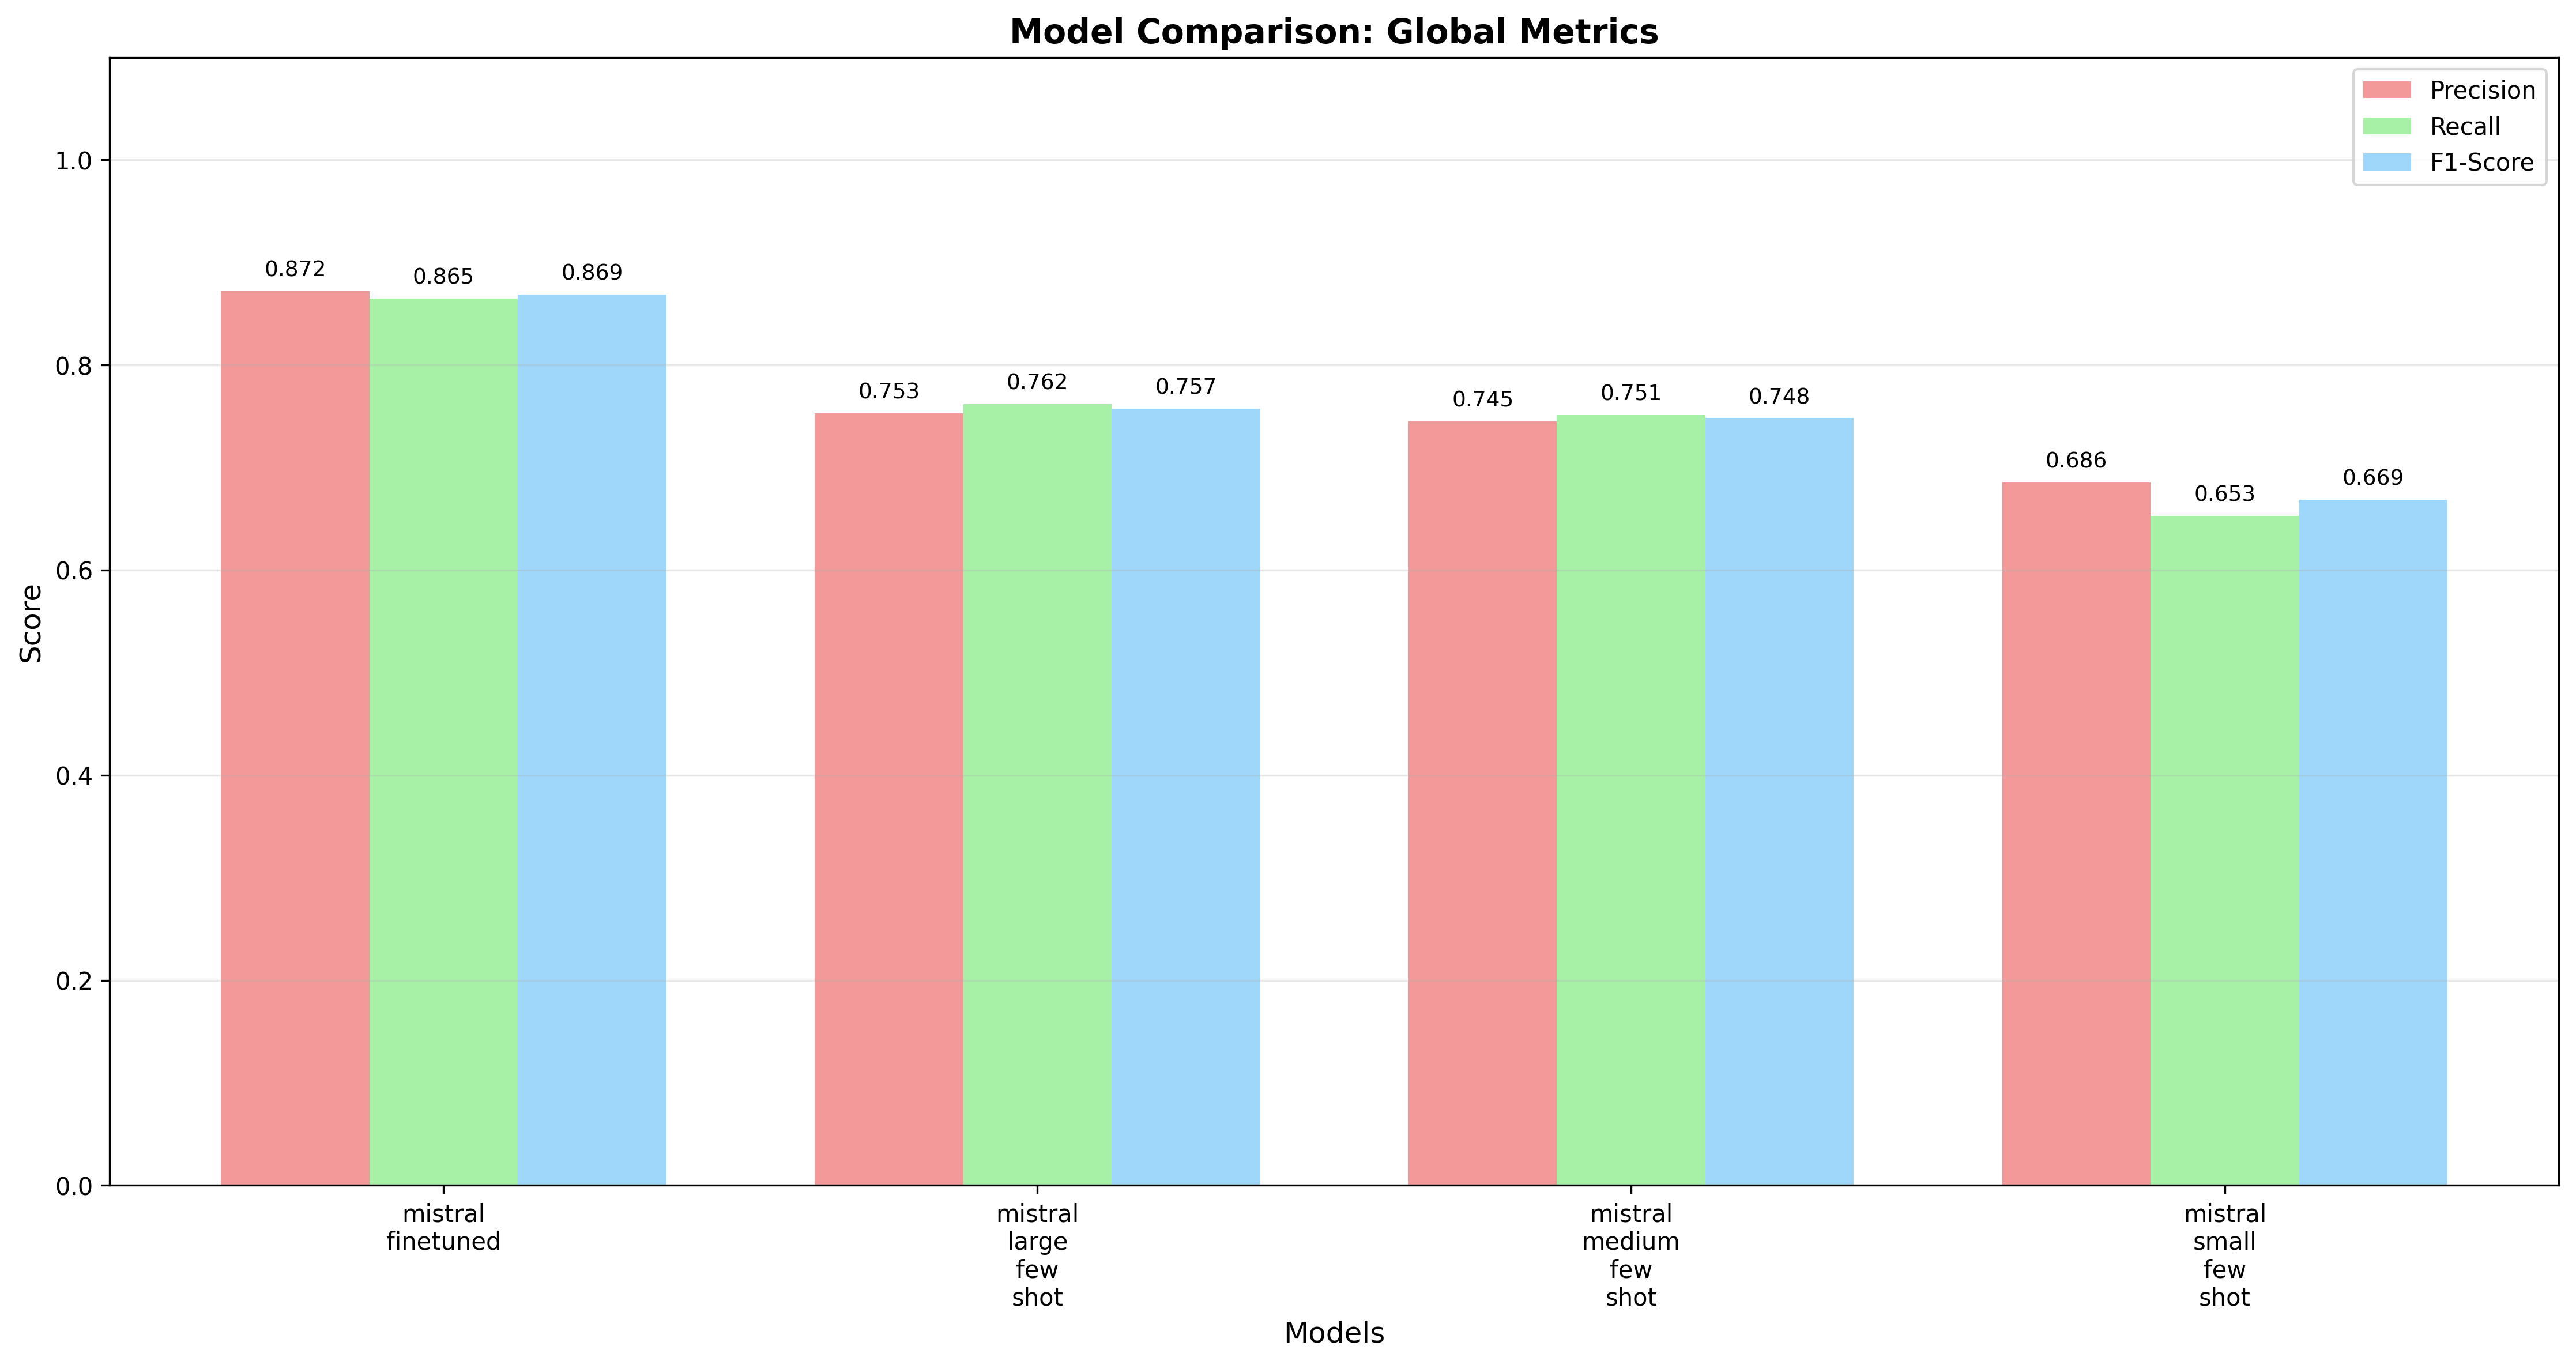
\includegraphics[width=0.8\textwidth]{images/model_comparison.png}
\end{center}
\end{table}

\begin{alertblock}{Key Insight}
Fine-tuning achieves \textbf{+4.5\% F1-score} improvement over few-shot prompting and is faster at inference time.
\end{alertblock}
\end{frame}

\section{Approach 3: Token Classification}

\begin{frame}{BERT Token Classification Approach}
\begin{columns}
\begin{column}{0.6\textwidth}
\textbf{Why Token Classification?}
\begin{itemize}
\item \textbf{Lightweight}: 66M vs 8B+ parameters
\item \textbf{Bidirectional}: Full context understanding
\item \textbf{CPU-Optimized}: No GPU requirements
\item \textbf{Fast Inference}: <100ms per document
\item \textbf{Specialized}: Purpose-built for NER tasks
\end{itemize}

\vspace{0.3cm}
\textbf{Architecture}
\begin{itemize}
\item Base: DistilBERT (distilled BERT-base)
\item Classification head: Linear layer per token
\item Subword tokenization with alignment
\end{itemize}
\end{column}
\begin{column}{0.4\textwidth}
\begin{center}
\includegraphics[width=\textwidth]{images/bert_architecture.png}
\caption{BERT Token Classification}
\end{center}

\vspace{0.3cm}
\begin{block}{vs. LLM Approaches}
\textbf{Pros:}
\begin{itemize}
\item 100x faster inference
\item No API dependencies
\item Offline deployment
\end{itemize}
\textbf{Cons:}
\begin{itemize}
\item Requires training data
\item Less flexible for new domains
\end{itemize}
\end{block}
\end{column}
\end{columns}
\end{frame}

\begin{frame}{BERT Training Results: Two Models Compared}
\begin{columns}
\begin{column}{0.5\textwidth}
\begin{center}
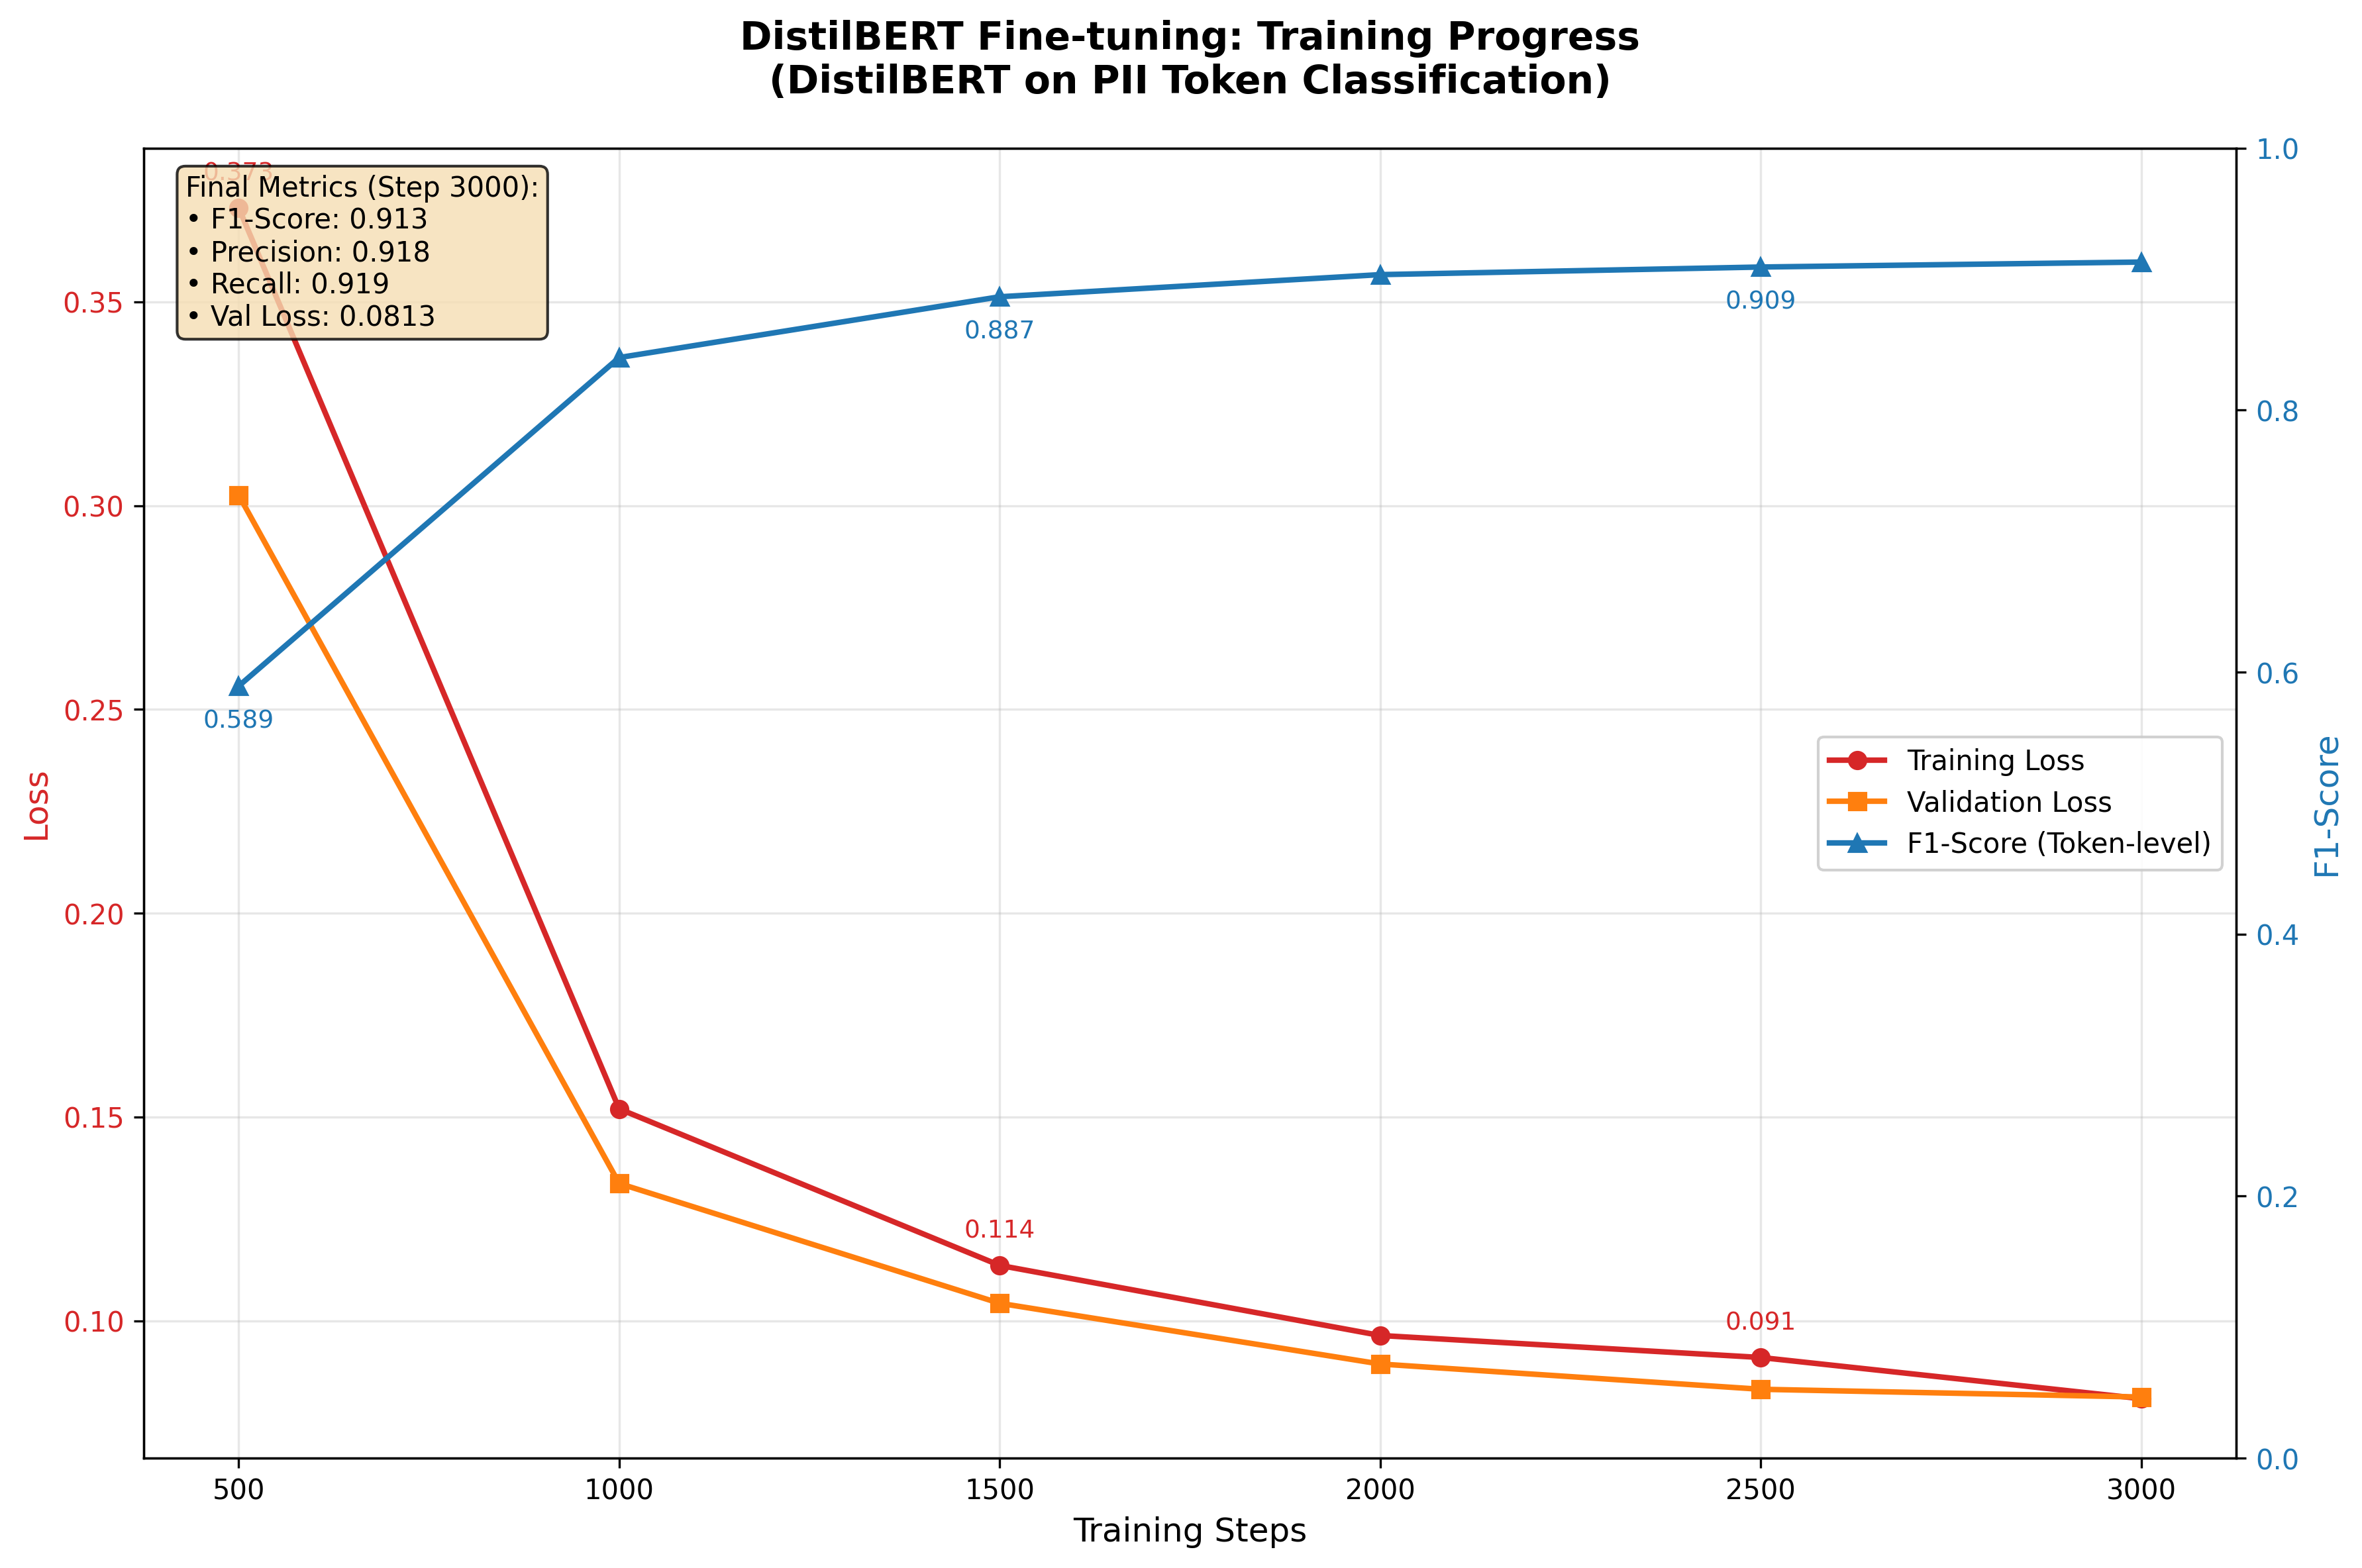
\includegraphics[width=\textwidth]{images/bert_distilled_training_loss.png}
\caption{DistilBERT Training}
\end{center}

\textbf{DistilBERT Performance}
\begin{itemize}
\item Token-level F1: \textbf{91.3\%}
\item Parameters: 66M
\item Training time: 3 epochs
\end{itemize}
\end{column}
\begin{column}{0.5\textwidth}
\begin{center}
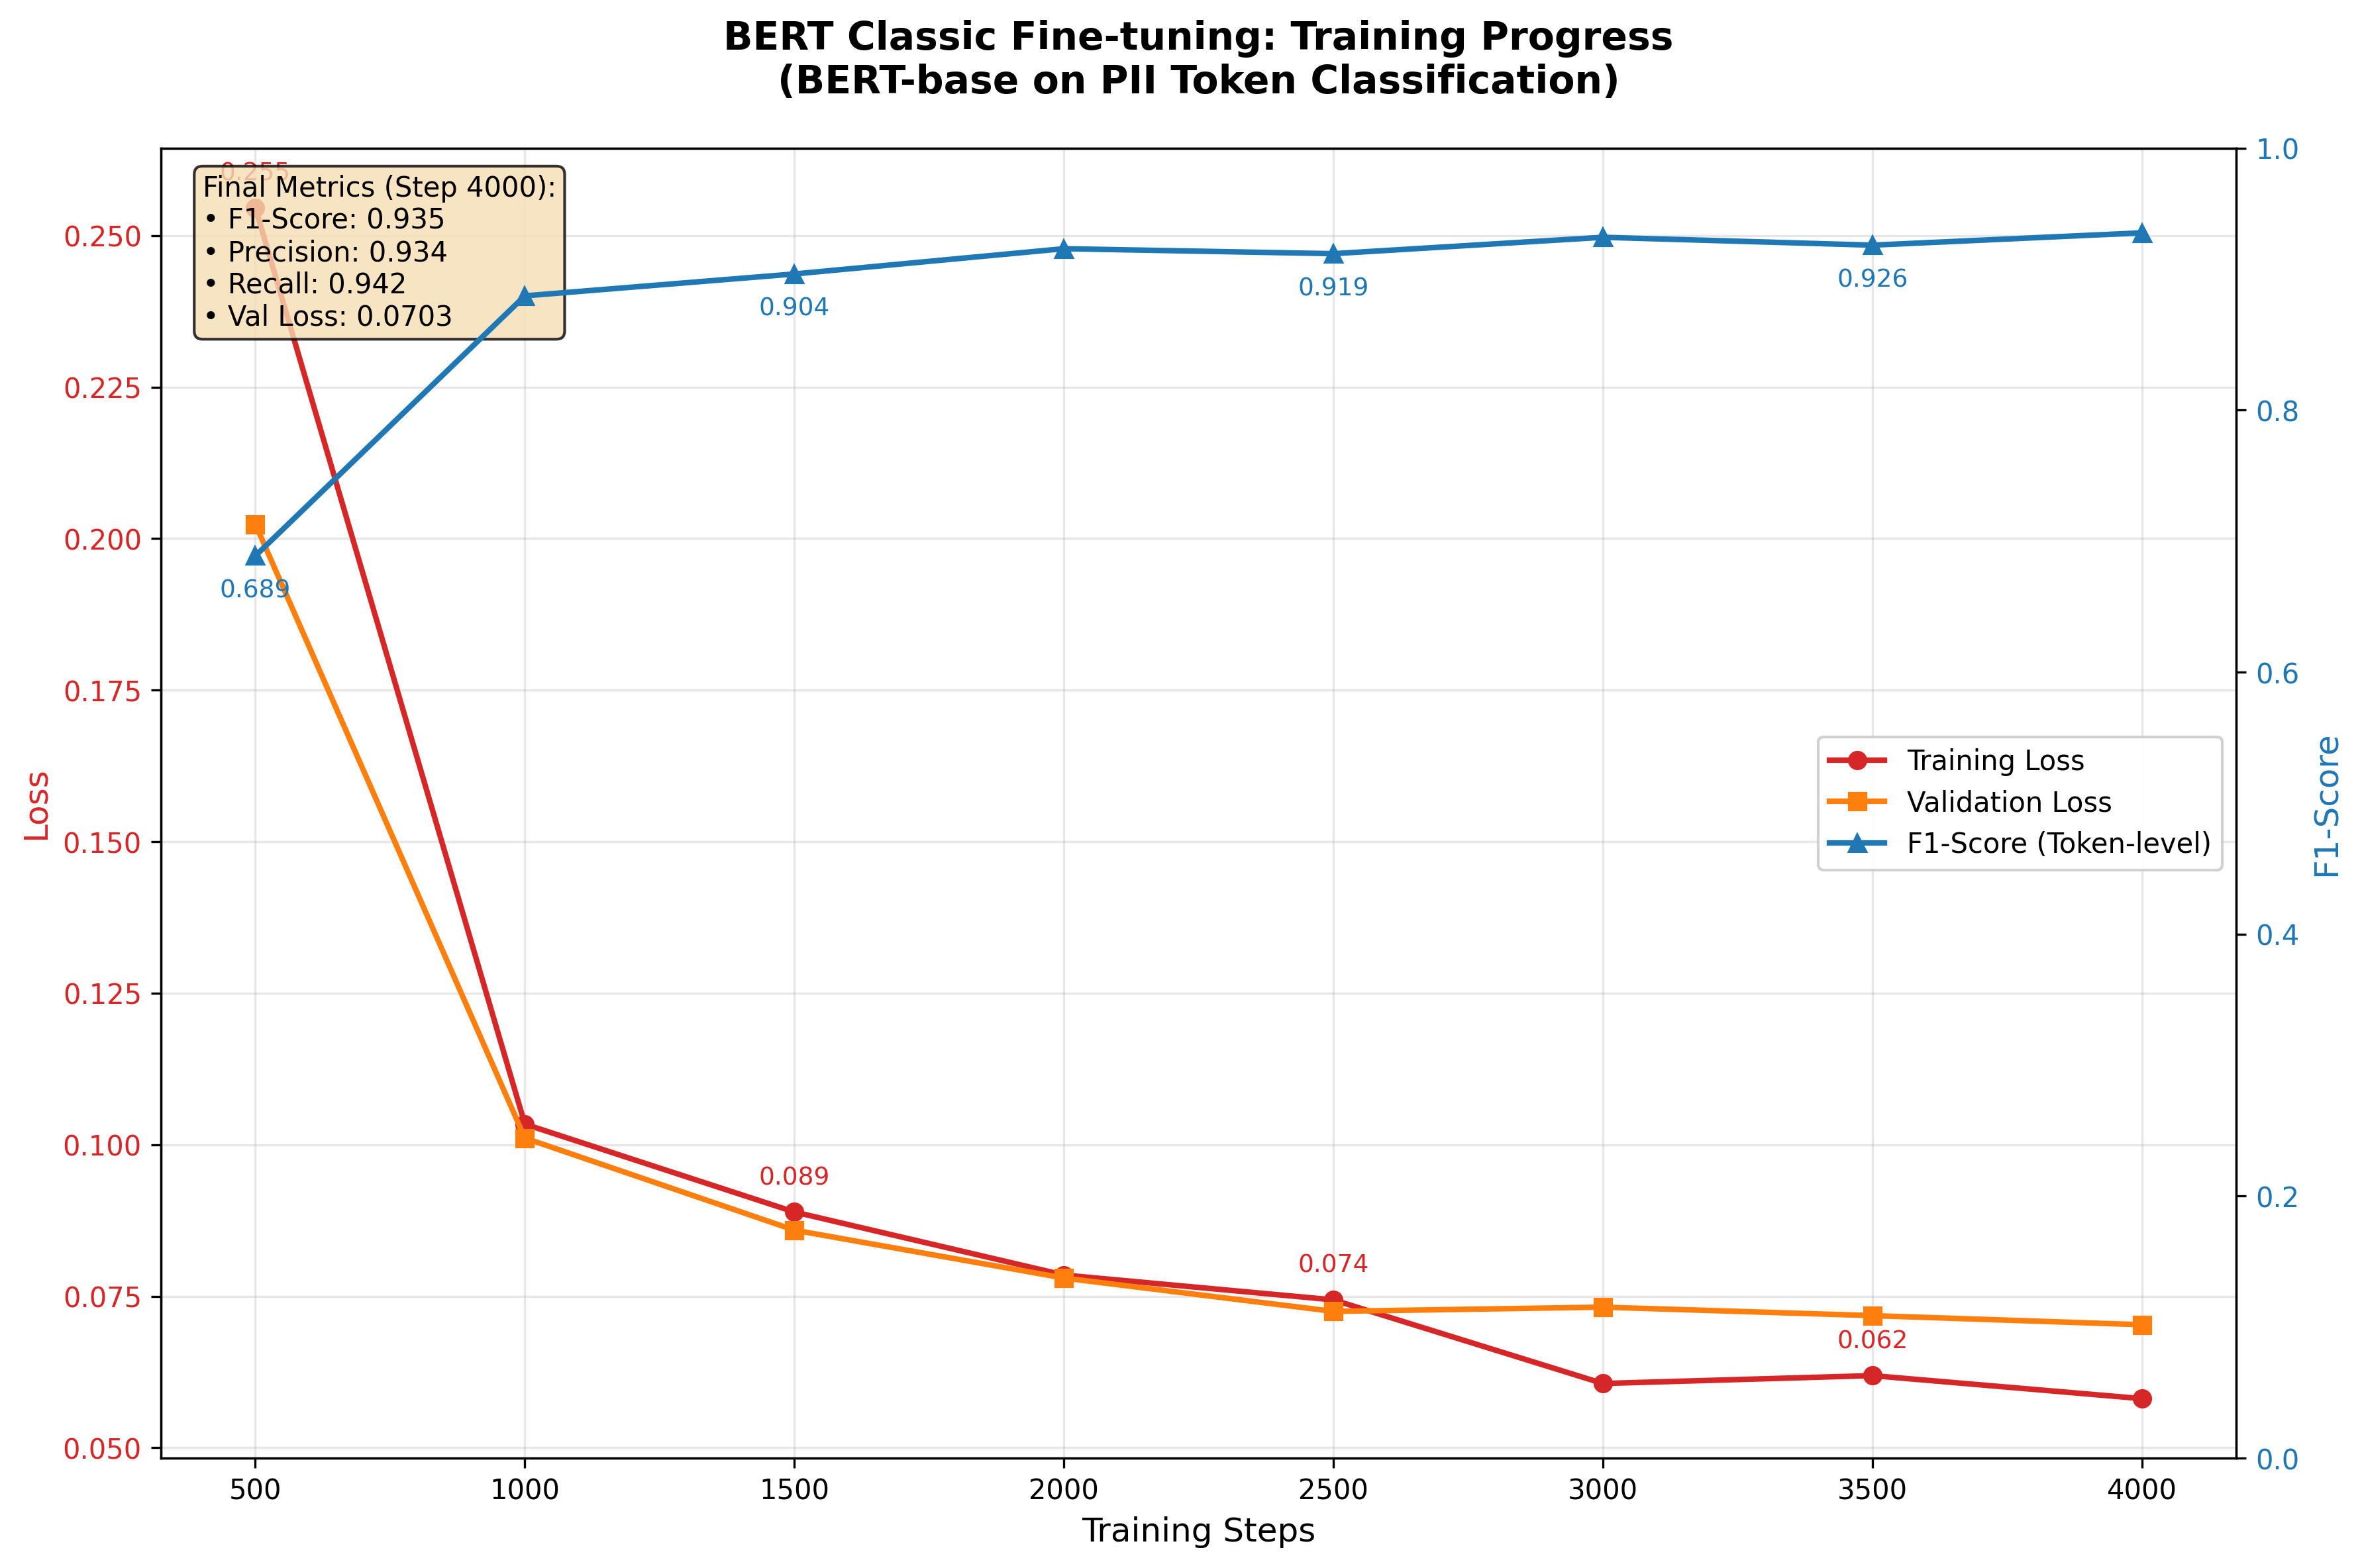
\includegraphics[width=\textwidth]{images/bert_classic_training_loss.png}
\caption{BERT Classic Training}
\end{center}

\textbf{BERT Classic Performance}
\begin{itemize}
\item Token-level F1: \textbf{93.5\%}
\item Parameters: 110M
\item Training time: 4 epochs
\end{itemize}
\end{column}
\end{columns}

\vspace{0.3cm}
\begin{alertblock}{Training Observation}
Both BERT models achieve excellent token-level performance (>91\%), but entity-level evaluation reveals different results...
\end{alertblock}
\end{frame}

\begin{frame}{Entity-Level Reality Check: The Performance Gap}
\begin{columns}
\begin{column}{0.5\textwidth}
\textbf{Token-Level Classification}
\begin{itemize}
\item Each token gets a BIO label
\item High accuracy: 91-93\% F1-score
\item Looks excellent during training
\item Standard NER evaluation
\end{itemize}

\vspace{0.3cm}
\textbf{Entity-Level Results}
\begin{itemize}
\item \textbf{BERT Classic}: 71.4\% F1
\item \textbf{DistilBERT}: 61\% F1
\item Gap: 20-30\% performance drop!
\end{itemize}
\end{column}
\begin{column}{0.5\textwidth}
\textbf{Why the Gap Exists}
\begin{itemize}
\item Token misalignment within entities
\item Boundary detection errors
\item Subword tokenization issues
\item Single token error = entire entity failed
\end{itemize}

\vspace{0.3cm}
\textbf{Example: Entity Failure}
\begin{center}
\texttt{John | Smith | lives | at}\\
\texttt{B-NAME | O | O | O}\\
\textcolor{red}{✗ Entity "John Smith" missed}
\end{center}
\end{column}
\end{columns}

\vspace{0.3cm}
\begin{alertblock}{Key Insight}
\textbf{Token-level metrics can be misleading!} BERT Classic achieves 71.4\% entity-level F1 vs 93.5\% token-level, showing why LLM approaches with JSON output perform better for real-world PII masking.
\end{alertblock}
\end{frame}

\begin{frame}{Complete Performance Comparison: All Methods}
\begin{center}
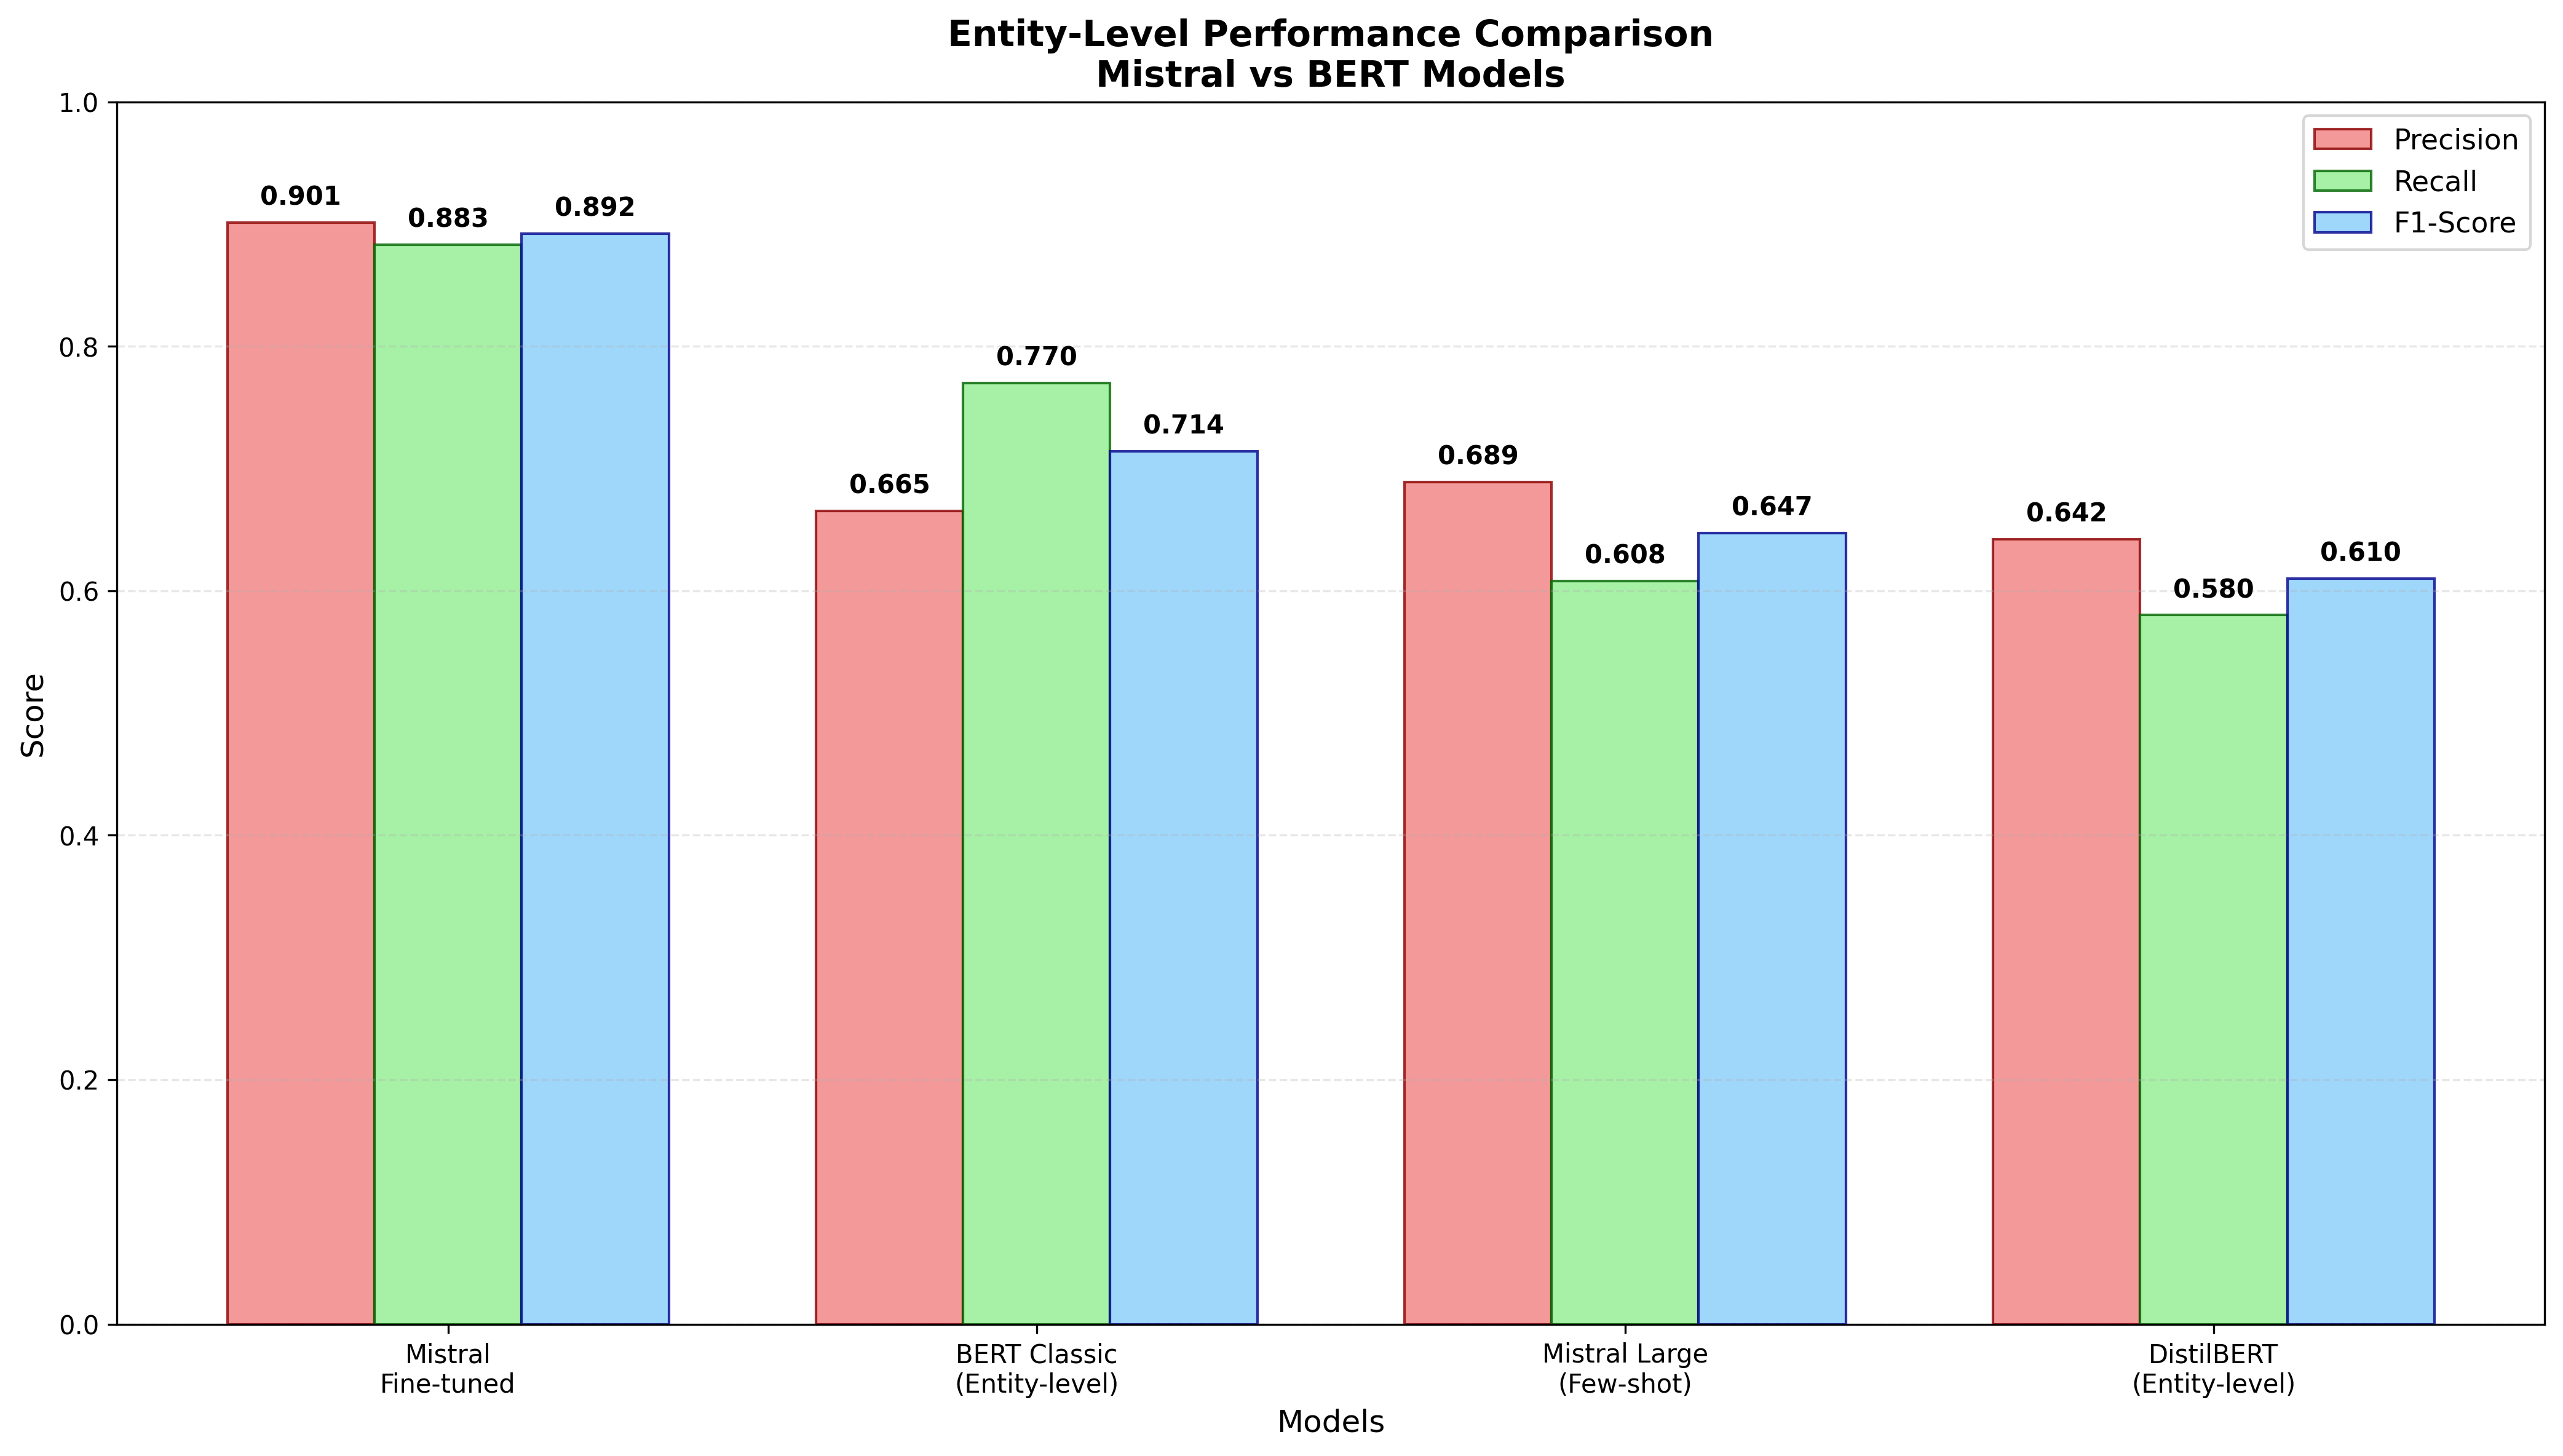
\includegraphics[width=0.9\textwidth]{images/bert_mistral_entity_comparison.png}
\end{center}

\vspace{0.3cm}
\begin{table}[h]
\centering
\scriptsize
\begin{tabular}{lcccc}
\toprule
\textbf{Method} & \textbf{Entity F1} & \textbf{Precision} & \textbf{Recall} & \textbf{Inference Time} \\
\midrule
Mistral Fine-tuned & \textbf{0.892} & \textbf{0.901} & 0.883 & 2.3s \\
BERT Classic & 0.714 & 0.665 & \textbf{0.770} & 89ms \\
Mistral Large (Few-shot) & 0.647 & 0.689 & 0.608 & 3.1s \\
DistilBERT & 0.610 & 0.642 & 0.580 & 45ms \\
\bottomrule
\end{tabular}
\end{table}

\begin{alertblock}{Key Findings}
\textbf{Both BERT Classic and Mistral Fine-tuned outperform Mistral Large Few-shot}, but Mistral Fine-tuned remains superior for entity-level accuracy. BERT Classic offers the best speed/accuracy trade-off.
\end{alertblock}
\end{frame}

\section{Production Solution}

\begin{frame}{Containerized Solution \& Deployment}
\begin{columns}
\begin{column}{0.5\textwidth}
\textbf{HuggingFace Space Deployment}
\begin{itemize}
\item \textbf{Live Demo}: huggingface.co/spaces/SoelMgd/pii\_masking
\item \textbf{Multi-method Support}: All 3 approaches available
\item \textbf{PDF Processing}: Drag-and-drop with OCR
\item \textbf{Entity Selection}: Granular PII type control
\item \textbf{Real-time Processing}: WebSocket updates
\end{itemize}

\vspace{0.3cm}
\textbf{Key Features}
\begin{itemize}
\item Modern UI
\item Batch processing capabilities
\item Export masked documents
\end{itemize}
\end{column}
\begin{column}{0.5\textwidth}
\begin{center}
\includegraphics[width=\textwidth]{images/frontend_demo.png}
\caption{Web Interface Screenshot}
\end{center}
\end{column}
\end{columns}
\end{frame}

\begin{frame}{System Architecture}
\begin{center}
\includegraphics[width=0.95\textwidth]{images/architecture_diagram.png}
\end{center}

\vspace{0.3cm}
\textbf{Component Overview}
\begin{itemize}
\item \textbf{Frontend}: HTML/JS with drag-and-drop PDF upload
\item \textbf{FastAPI Backend}: Async processing with different inference services
\item \textbf{BERT Service}: CPU-optimized local inference (HuggingFace Hub)
\item \textbf{Mistral Services}: Chunking and batch processing to speed up long text inderence
\item \textbf{OCR Service}: Mistral OCR for PDF text extraction
\end{itemize}
\end{frame}

\begin{frame}{Smart Async/Sync Architecture: Handling Concurrency}
\begin{columns}
\begin{column}{0.5\textwidth}
\textbf{The Challenge}
\begin{itemize}
\item \textbf{BERT}: CPU-bound (blocking operations)
\item \textbf{Mistral}: I/O-bound (network calls)
\item \textbf{FastAPI}: Async framework
\item \textbf{Goal}: Serve multiple users simultaneously
\end{itemize}

\vspace{0.3cm}
\textbf{Naive Approach Problems}
\begin{itemize}
\item BERT blocks entire event loop
\item Users wait sequentially
\item Poor scalability under load
\end{itemize}
\end{column}
\begin{column}{0.5\textwidth}
\textbf{Our Solution: Unified Interface}
\begin{lstlisting}[language=python,basicstyle=\tiny]
class BasePIIInferenceService:
    async def predict(self, text):
        # Auto-routing based on service type
        try:
            # Try native async (Mistral)
            return await self.predict_async_native(text)
        except NotImplementedError:
            # Fall back to thread pool (BERT)
            return await asyncio.to_thread(
                self.predict_sync, text
            )
\end{lstlisting}

\vspace{0.3cm}
\textbf{Benefits}
\begin{itemize}
\item \textbf{BERT}: Runs in thread pool (non-blocking)
\item \textbf{Mistral}: Native async (I/O efficient)
\item \textbf{FastAPI}: Unified \texttt{await} interface
\item \textbf{Concurrency}: Multiple requests served simultaneously
\end{itemize}
\end{column}
\end{columns}
\end{frame}

\begin{frame}{Concurrency Performance Demonstration}
\begin{columns}
\begin{column}{0.6\textwidth}
\begin{center}
\includegraphics[width=\textwidth]{images/concurrency_comparison.png}
\caption{Sequential vs Concurrent Request Handling}
\end{center}
\end{column}
\begin{column}{0.4\textwidth}
\textbf{Sequential (Bad)}
\begin{itemize}
\item Request 1: BERT (2s)
\item Request 2: Mistral (3s) \textit{waits}
\item Request 3: BERT (2s) \textit{waits}
\item \textbf{Total: 7 seconds}
\end{itemize}

\vspace{0.3cm}
\textbf{Concurrent (Good)}
\begin{itemize}
\item Request 1: BERT (2s) \textit{in thread}
\item Request 2: Mistral (3s) \textit{async}
\item Request 3: BERT (2s) \textit{in thread}
\item \textbf{Total: 3 seconds}
\end{itemize}

\vspace{0.3cm}
\begin{alertblock}{Performance Gain}
\textbf{2.3x faster} under concurrent load\\
Multiple users served simultaneously
\end{alertblock}
\end{column}
\end{columns}
\end{frame}

\begin{frame}{Technical Implementation: Service Pattern Design}
\begin{columns}
\begin{column}{0.5\textwidth}
\textbf{BERT Service (CPU-bound)}
\begin{lstlisting}[language=python,basicstyle=\tiny]
class BERTInferenceService(BasePIIInferenceService):
    def predict_sync(self, text):
        # Synchronous PyTorch operations
        inputs = self.tokenizer(text, ...)
        with torch.no_grad():
            outputs = self.model(**inputs)
        return self.process_predictions(outputs)
    
    # predict() inherited from base class
    # Automatically wraps with asyncio.to_thread()
\end{lstlisting}

\vspace{0.3cm}
\textbf{Mistral Service (I/O-bound)}
\begin{lstlisting}[language=python,basicstyle=\tiny]
class MistralPromptingService(BasePIIInferenceService):
    async def predict_async_native(self, text):
        # Native async API calls
        response = await self.client.chat(
            messages=[{"role": "user", "content": text}]
        )
        return self.process_json_response(response)
    
    # predict() inherited from base class
    # Calls predict_async_native() directly
\end{lstlisting}
\end{column}
\begin{column}{0.5\textwidth}
\textbf{FastAPI Integration}
\begin{lstlisting}[language=python,basicstyle=\tiny]
@app.post("/predict")
async def predict(request: PredictionRequest):
    if request.method == "bert":
        # BERT: sync -> thread pool
        prediction = await bert_service.predict(text)
    elif request.method == "mistral":
        # Mistral: native async
        prediction = await mistral_service.predict(text)
    
    return PredictionResponse(
        masked_text=prediction.masked_text,
        entities=prediction.entities,
        processing_time=processing_time
    )
\end{lstlisting}

\vspace{0.3cm}
\textbf{Key Advantages}
\begin{itemize}
\item \textbf{Unified Interface}: Same \texttt{await} call for all services
\item \textbf{Automatic Routing}: Service type determines execution pattern
\item \textbf{Zero Blocking}: Event loop never blocked
\item \textbf{Scalable}: Handles concurrent users efficiently
\item \textbf{Maintainable}: Clean separation of concerns
\end{itemize}
\end{column}
\end{columns}
\end{frame}

\begin{frame}{Performance \& Inference Time Analysis}
\begin{center}
\includegraphics[width=0.8\textwidth]{images/inference_times.png}
\end{center}

\begin{table}[h]
\centering
\begin{tabular}{lccc}
\toprule
\textbf{Method} & \textbf{Single Doc} & \textbf{Batch (10 docs)} & \textbf{Cost per 1k docs} \\
\midrule
DistilBERT (CPU) & 45ms & 180ms & \$0.00 \\
BERT-base (CPU) & 89ms & 340ms & \$0.00 \\
Fine-tuned Mistral & 2.3s & 8.2s & \$15.00 \\
Mistral-large API & 3.1s & 12.4s & \$80.00 \\
\bottomrule
\end{tabular}
\end{table}

\begin{alertblock}{Deployment Recommendation}
\textbf{Mistral Fine-tuned leads in accuracy (89.2\%)} but BERT Classic provides excellent speed/accuracy trade-off (71.4\% F1, 25x faster). Both outperform Mistral Large Few-shot (64.7\%).
\end{alertblock}
\end{frame}

\begin{frame}{Codebase Structure \& Extensibility}
\begin{columns}
\begin{column}{0.5\textwidth}
\textbf{Modular Framework}
\begin{itemize}
\item \texttt{src/pii\_masking/}: Core library
\item \texttt{experiments/}: Research implementations  
\item \texttt{space/}: Production deployment
\end{itemize}

\vspace{0.3cm}
\textbf{Key Design Principles}
\begin{itemize}
\item Abstract base classes for extensibility
\item Standardized evaluation pipeline
\item Configuration-driven experiments
\item Reproducible results
\end{itemize}
\end{column}

\vspace{0.2cm}
\textbf{Standardized Evaluation}
\begin{itemize}
\item Consistent metrics across approaches
\item Per-class performance analysis
\item Export results to JSON/CSV
\item Visualization utilities included
\end{itemize}
\end{columns}
\end{frame}

\section{Conclusions \& Future Work}

\begin{frame}{Key Findings \& Recommendations}
\begin{columns}
\begin{column}{0.5\textwidth}
\textbf{Performance Summary}
\begin{enumerate}
\item \textbf{Mistral Fine-tuned}: Highest accuracy (89.2\% F1)
\item \textbf{BERT Classic}: Strong performance (71.4\% F1), 25x faster
\item \textbf{Mistral Large Few-shot}: Good baseline (64.7\% F1)
\item \textbf{DistilBERT}: Fastest but limited (61\% F1)
\end{enumerate}

\vspace{0.3cm}
\textbf{Business Recommendations}
\begin{itemize}
\item \textbf{Maximum accuracy}: Mistral Fine-tuned
\item \textbf{Best speed/accuracy}: BERT Classic fine-tuned
\item \textbf{Rapid deployment}: Mistral Few-shot prompting
\item \textbf{High-volume/cost-sensitive}: DistilBERT (with trade-offs)
\end{itemize}
\end{column}
\begin{column}{0.5\textwidth}
\textbf{Technical Achievements}
\begin{itemize}
\item Comprehensive evaluation framework
\item Production-ready deployment
\item Multi-method comparison
\item Cost-effective batch processing
\item \textbf{Smart async/sync architecture} for optimal concurrency
\end{itemize}

\vspace{0.3cm}
\begin{alertblock}{ROI Impact}
Framework enables data-driven decisions between \textbf{accuracy}, \textbf{cost}, and \textbf{speed} based on specific business requirements.
\end{alertblock}
\end{column}
\end{columns}
\end{frame}

\begin{frame}{Future Work \& Extensions}
\begin{columns}
\begin{column}{0.5\textwidth}
\textbf{Model Improvements}
\begin{itemize}
\item \textbf{Ensemble Methods}: Combine BERT + Mistral predictions
\item \textbf{Domain Adaptation}: Sector-specific fine-tuning
\item \textbf{Multilingual Support}: Extend to other languages
\end{itemize}
\end{column}
\begin{column}{0.5\textwidth}
\textbf{Business Applications}
\begin{itemize}
\item \textbf{Document Intelligence}: Contract analysis pipelines
\item \textbf{Compliance Automation}: GDPR data discovery
\item \textbf{Data Lake Sanitization}: Enterprise data governance
\item \textbf{Customer Onboarding}: KYC document processing
\end{itemize}

\end{column}
\end{columns}
\end{frame}

\begin{frame}{Thank You}
\begin{center}
{\Large \textbf{Questions \& Discussion}}

\vspace{1cm}

\textbf{Live Demo Available:}\\
\href{https://huggingface.co/spaces/SoelMgd/pii_masking}{huggingface.co/spaces/SoelMgd/pii\_masking}

\vspace{0.5cm}

\textbf{Repository:}\\
\href{https://github.com/username/pii-masking-200k}{github.com/username/pii-masking-200k}

\vspace{1cm}

\textit{Demonstrating systematic AI evaluation combining technical rigor with business pragmatism - essential skills for Applied AI Engineering at Mistral AI.}
\end{center}
\end{frame}

\end{document} 